\documentclass{article}


\usepackage{arxiv}

\usepackage[utf8]{inputenc} % allow utf-8 input
\usepackage[T1]{fontenc}    % use 8-bit T1 fonts
\usepackage{hyperref}       % hyperlinks
\usepackage{url}            % simple URL typesetting
\usepackage{booktabs}       % professional-quality tables
\usepackage{amsfonts}       % blackboard math symbols
\usepackage{nicefrac}       % compact symbols for 1/2, etc.
\usepackage{microtype}      % microtypography
\usepackage{lipsum}
\usepackage[nottoc]{tocbibind}
\usepackage{graphicx}
\usepackage{titlesec}

\titlespacing{\section}{0pt}{\parskip}{-\parskip}
\titlespacing{\subsection}{0pt}{\parskip}{-\parskip}
\titlespacing{\subsubsection}{0pt}{\parskip}{-\parskip}


\title{On Road Vehicle Detection using \emph{Classical Machine Learning} Techniques}


\author{
  Pratyush Kumar \\
  Department of Computer Science\\
  Ashoka University\\
  Sonipat, Haryana \\
  \texttt{pratyush.kumar\textunderscore ug21@ashoka.edu.in} \\
  %% examples of more authors
   \And
 Vedansh Priyadarshi \\
  Department of Computer Science\\
  Ashoka University\\
  Sonipat, Haryana \\
  \texttt{vedansh.priyadarshi\textunderscore ug21@ashoka.edu.in} \\
 \AND
  Shekhar Chaterjee \\
  Department of Computer Science \\
  Ashoka University \\
  \texttt{shekhar.chaterjee\textunderscore ug20@ashoka.edu.in} \\
  %% \And
  %% Coauthor \\
  %% Affiliation \\
  %% Address \\
  %% \texttt{email} \\
  %% \And
  %% Coauthor \\
  %% Affiliation \\
  %% Address \\
  %% \texttt{email} \\
}

\begin{document}
\maketitle
\begin{abstract}
On road vehicle detection has been an interesting and challenging area of research in Machine Learning and Computer Vision. Over the years, the field of machine learning has grown from using conventional techniques to using modern Deep Learning techniques like Recurrent Neural Network\cite{1808-03314} and semantic image segmentation\cite{1412.7062} techniques. Approaches described in papers like YOLO \cite{1506.02640}, are the current state-of-the-art in object recognition. In this project, we use Histogram of Gradients(HOG)\cite{1501.02058} and run experiments to explore the nuances and features this method uses to differentiate between objects. We apply this to detecting cars and train four models namely Multi-Layers Perceptron\cite{1412.5513}, Decision Trees\cite{1305.4537}, Naive Bayes\cite{1302.5189} and Support Vector Machines\cite{1506.02509}. To test the model, we draw boxes in frames where ever a vehicle is detected and qualitatively decide if a particular model is performing well. 
\end{abstract}


% keywords can be removed
\keywords{HOG}


\section{Related Work}
There are extensive literature on object detection, but here we mention just a few relevant papers on vehicle detection. Ding et al.\cite{1802.03515} presented an accurate approach to estimate vehicle pose using CNNs by extracting vehicles’ semantic keypoints. Satar et al.\cite{1809.00953} proposed to combine an SSD (Single Shot Multibox Detector) model with a CNN (Convolutional Neural Network) model to train on the database. There are lots of work that has been done on vehicle re-identification by using deep learning techniques. Alfasly et al.\cite{1905.02343} presented two-fold framework by using variational feature learning and long short-term memory (LSTM) to learn the relationship among different viewpoints of a vehicle. Oliveira et al.\cite{1911.05541} proposed Two-Stream Siamese Neural Network for vehicle re-identification. Sheeny et al.\cite{1804.02576} proposed a method of vehicle detection using polarised long wave infrared sensors and Faster-RCNN. Hu et al.\cite{1804.00433} presented state-of-the-art SINet, which is a scale-insensitive Convolutional Neural Network (CNN) for fast vehicle detection. Moghimi er al.\cite{1801.01698} presented a method for moving vehicle detection using AdaBoost and Haar-Like features in surveillance videos. Recently, Fu et al.\cite{1910.01701} presented low-cost LIDAR based vehicle pose estimation and tracking.

\section{Approach}
In our approach to solving this problem, we started with a statement that in order to indentify vehicles, our model must be capable of differentiating vehicles from other non-vehicle objects present on road. In order to obtain such a model, a dataset from GIT\cite{Arrspide2012} and KITI\cite{Fritsch2013ITSC} consisting of vehicle and non-vehicle images was used. The images in the dataset are of size $64\times64$. Below is the visualization of a random sample from the dataset:

\begin{figure}[h]
\centering
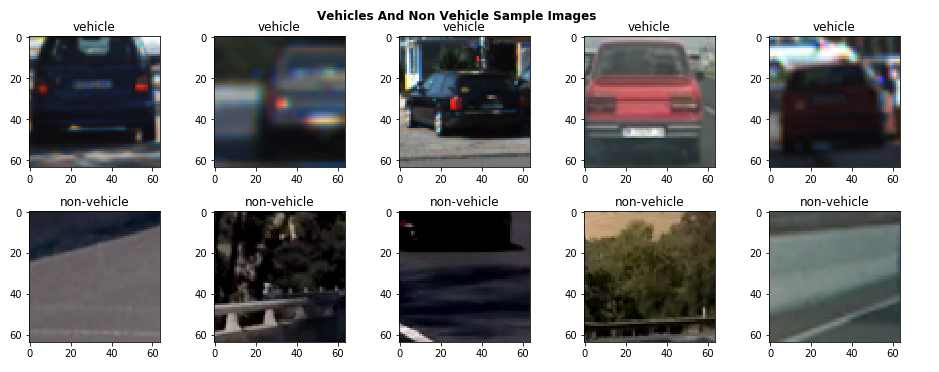
\includegraphics[width=\textwidth]{plots_pics.png}
\caption{Dataset Visualization}
\end{figure}

Images contain information about the color, orientation among other assortment of data and the question arises as to how can the best features be extracted from the images so that our models are able to best learn to classify between vehicles and non-vehicles. A viable approach will be to extract features that contain information about the shape and size of the car. For this we use the Histogram of Gradients (HOG) \cite{1501.02058} algorithm.

\subsection{Histogram of Gradients}
Calculating the histogram of gradients of an image involves the following steps:\\
$1.)$ Normalization and equalization of whole image. This is performed by either either computing the square root or the log of each color channel\cite{1501.02058}. This step helps reduce the effects from local shadowing and illumination variations.\\
$2.)$ Calculate the gradients along \textbf{x} and \textbf{y} axis: This is done by first filtering the image with the help of two kernels shown in Fig. 2

\begin{figure}[h]
\centering
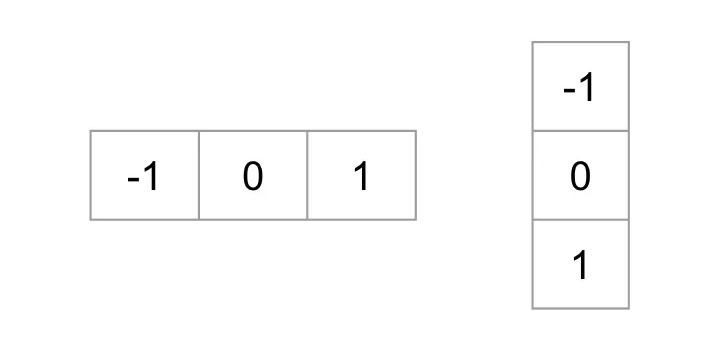
\includegraphics[width=\textwidth]{kernel.png}
\caption{Sobel operator filter\cite{mallick_2016}}
\end{figure}

This technically employs the Sobel operator\cite{1910.00138} to detect edges. Following this, the magnitude and direction of gradient is calculated using the formulas   $Gradient = \sqrt{g_x^2+g_y^2} \hspace{20pt}$   $\theta = arctan\frac{g_y}{g_x}$
The output is an image that highlights all the edges of an object and removes a lot of non-essential information like constant colored background.

$3.)$Next, this algorithm calculates gradients across a patch of image of size $height\times width$ This is called the $\textbf{cell-size}$ The cell-size can be of any shape but using a small cell-size is recommended as it draws out a compact representation and is thus robust to noise. Consider a cell-size of $8\times8$ which will have $8\times8\times2 = 128$ numbers represented as an array of $9$ numbers (in case of unsigned gradients) and $18$ numbers (in case of signed gradients). Here, w multiply $8\times8$ with 2 as we will have two $8\times8$ matrices one representing gradients direction and the gradient magnitude.\\

$4.)$ Make the histograms: The way we make histograms is as follows: For unsigned gradients, the nine element array is used where each element represents the division of angles from $0-180$ degrees as : $0,20,40, .... , 180$. The image\cite{mallick_2016} shown below explains this better:

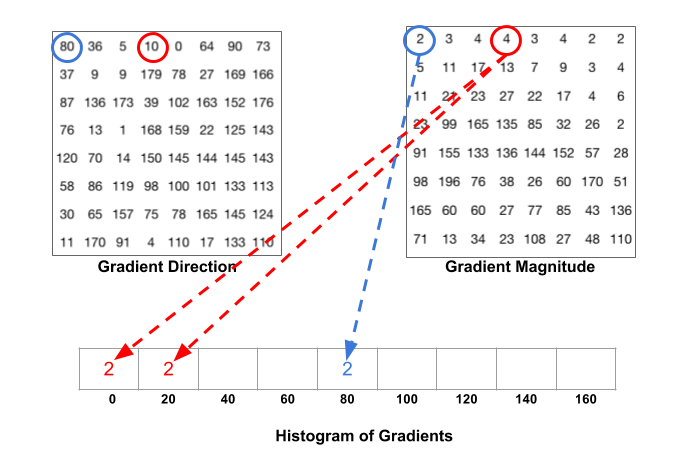
\includegraphics[width=\textwidth]{hog1.png}

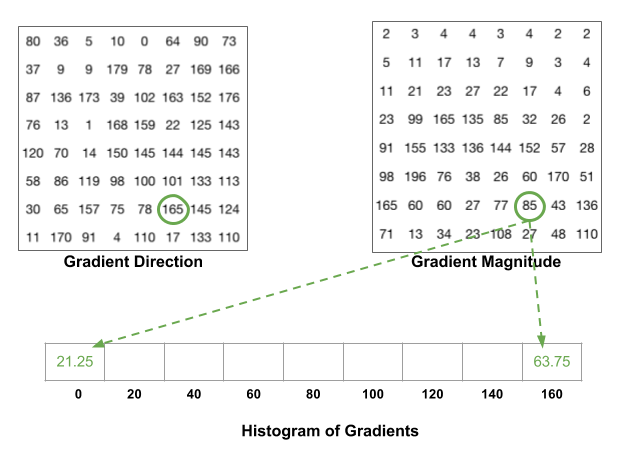
\includegraphics[width=\textwidth]{hog2.png}

The gradient direction decides, what cell of the $9$ available cells does the gradient magnitude goes into. If the direction value is equally placed between two cell values, the magnitude equally divides between the two cell. Another case is visualized above\cite{mallick_2016}:


If the direction is not mid-way between two values, the value is proportionally divided between the two cells.

$5.)$ Block Normalization: Finally, we take a block size larger than the cell-size say $16\times16$ for a cell-size of $8\times8$. We are just keeping the block-size larger than the initial size as this was the general practice followed in other implementations of the code we studied. In this method, we calculate the length of the histogram vector for each cell and place them one after the other horizontally to get a feature vector.

\subsection{Data Analysis}
In order to figure out the best hyper-parameters for calculating the HOG, we try out a couple most commonly used values for cell-size/ pixels per cell, block size, scale. Upon experimentation, we concluded that pixel-per-size of $14$ with block size of $2$ worked best for drawing out the best features.\\
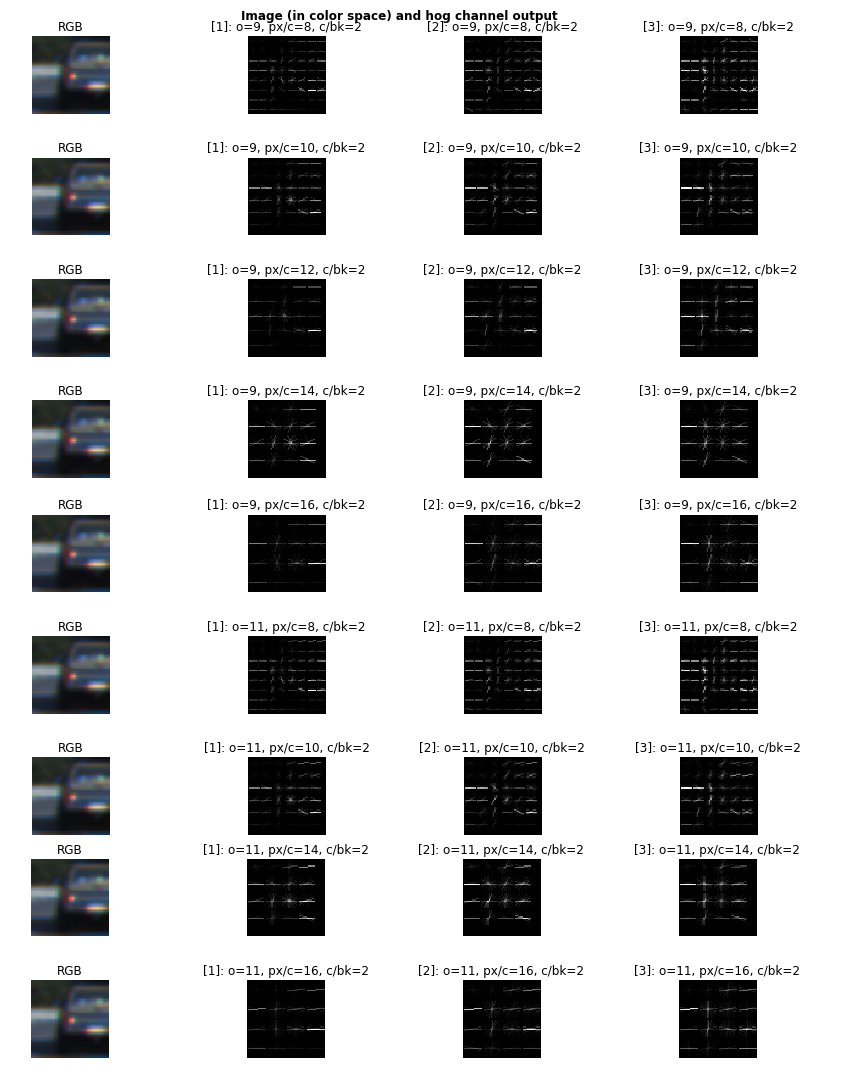
\includegraphics[width=\textwidth]{1.png}

In our approach, we calculated HOG along all three channels of the image separately in order to check if we can draw a mixture of features that might help improve the training process. We observed that $\textbf{RGB}$ gave similar features along all three channels. We tried other color channels like HSV, YUV, HLS, YCrCb, LAB. While other rest of the color channels were firing for arbitrary features, $\textbf{YCrCb}$ appeared to give varying, useful features across multiple images. So, we went ahead with this color channel.\\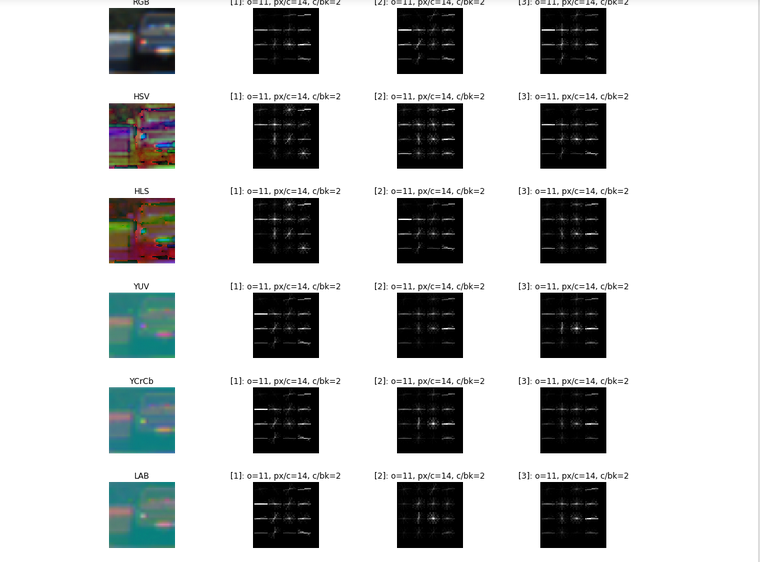
\includegraphics[width=\textwidth]{colors.png}
 We train our models on these features drawn on these parameters. While testing it out on provided test videos\cite{Sivaraman}, we used a strategy to take a $32\times32$ patch across each frame, drawing $10$ frames per sample. In order to check if the model is detecting vehicles, we implemented a method that saves the top-left and bottom-right co-ordinates of the patches in a frame and draws a rectangle around it. Methods were implemented to smooth the bounding boxes based on the centroid of the boxes so that the output in videos is a clean box. To get a clearer picture of what the model is doing, a method to visualize heap-map in areas where cars are detected by the model was also implemented.

\section{Results}
We trained out data set of $8792$ vehicles and $8968$ non-vehicles where a shuffled dataset of $14208$ data points made the training set and the rest were used for testing the model. Below is the accuracy of the model on both training and testing dataset:\bigbreak
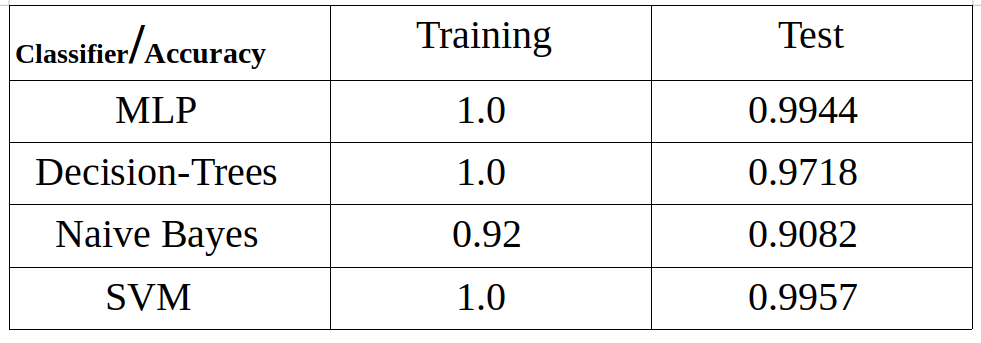
\includegraphics[width=\textwidth]{result.png}
The training process looked like: \bigbreak 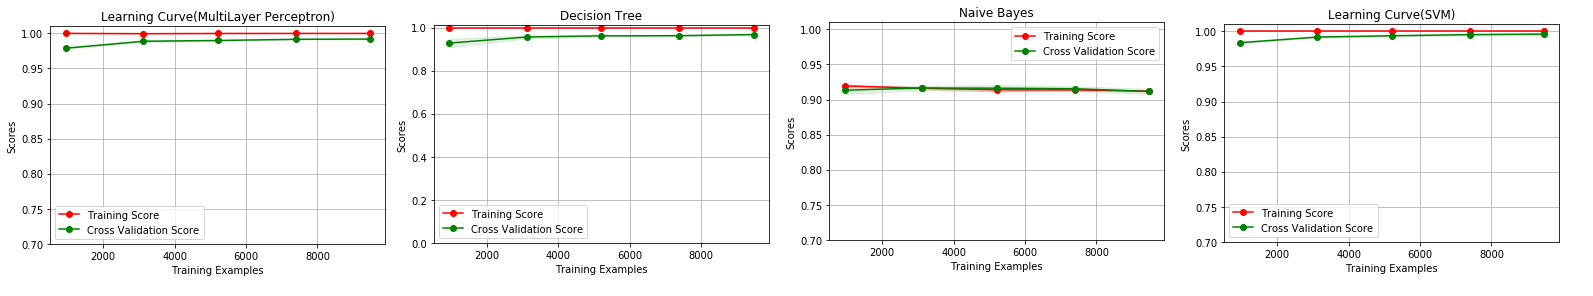
\includegraphics[width=\textwidth]{LearningCurve.png}

When tested on frames from the test videos, below are the results for different models: \bigbreak 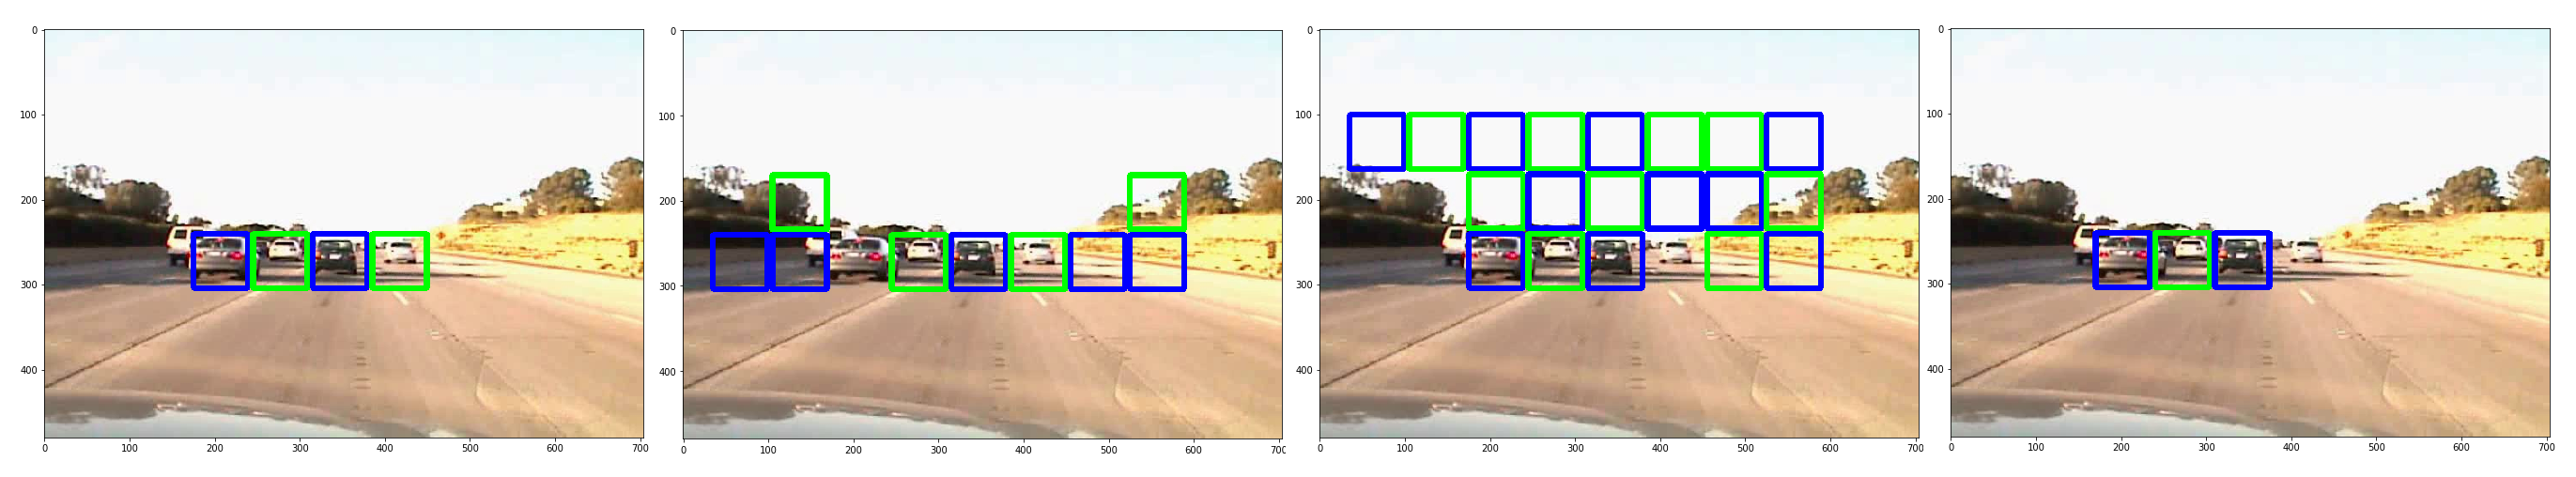
\includegraphics[width=\textwidth]{cars.png}

All the above images follow the order: \textbf{MLP, Decision Trees, Naive Bayes, SVM} The github repository with all code, files and results are: \url{https://github.com/Cloaked04/IML_Final_Project}

\section{Conclusion \& Future Work}
Detecting vehicles using HOG feature extraction technique gives descent results on the test videos. But the method involves hard-coding multiple steps that is a bottleneck in generalizing this technique. For instance, in order to obtain the right classification, we had to take the frame in the range of $100-200$ along the height so as to not include the sign board. Not doing so results in the mis-classification of the sign board as it resembles the number plates at the back of a car. 
The quality of video also plays a role in prediction, better pixel density allows for more data to be captured in the frames allowing for better features. The test video was simple-definition video with a lower pixel density. \\
Modern techniques in Deep Learning like \textbf{YOLO}, \textbf{Faster-RCNN} and others have given much better results on object detection tasks. These have been applied to Vehicle detection tasks and have given good results. In the future, we plan on implementing some state of the art models and combining them with segmentation\cite{1412.7062} techniques and experiment with the features in hope of improving our results.   

  %%% Remove comment to use the external .bib file (using bibtex).
%%% and comment out the ``thebibliography'' section.

\bibliographystyle{unsrt}  
\bibliography{references}

\end{document}
